\documentclass[10pt]{article}
\usepackage{graphicx} % Required for inserting images
\usepackage[a4paper,margin=2.2cm]{geometry}
\usepackage[ruled,vlined,linesnumbered]{algorithm2e}
\usepackage[T1]{fontenc}
\usepackage[utf8]{inputenc}
\usepackage{lmodern}
\usepackage{longtable}
\usepackage{microtype}
\usepackage{amsmath,amssymb,mathtools}
\usepackage{booktabs,tabularx,array,multirow}
\usepackage{enumitem}
\usepackage{appendix}
\usepackage{booktabs}
\usepackage{array}
\usepackage{xcolor}
\usepackage{tikz}
\usepackage{enumitem}
\usepackage{amsthm}
\usetikzlibrary{arrows.meta,
positioning,
fit,
shapes.geometric, 
backgrounds, 
calc}
\usepackage{listings}
\usepackage{hyperref}
\usepackage[nameinlink,noabbrev]{cleveref}
\usepackage{caption}
\usepackage{subcaption}
\usepackage{url}
\usepackage{balance}
\usepackage{tabularx}
\usepackage{booktabs}
\usepackage{array}
\usepackage{makecell}
\usepackage{ragged2e}
\newcolumntype{C}[1]{>{\Centering\arraybackslash}p{#1}}
\newcolumntype{Y}{>{\RaggedRight\arraybackslash}X}

\definecolor{acmblue}{RGB}{37,80,130}
\definecolor{acmgray}{RGB}{245,247,249}
\definecolor{passgreen}{RGB}{34,139,34}
\definecolor{deviationorange}{RGB}{210,105,30}
\definecolor{skipgray}{RGB}{105,105,105}
\definecolor{failred}{RGB}{178,34,34}
\definecolor{alertred}{RGB}{178,34,34}
\definecolor{preservedgreen}{RGB}{34,139,34}
\definecolor{approximatedorange}{RGB}{210,105,30}
\definecolor{unsupportedgray}{RGB}{105,105,105}
\hypersetup{
  colorlinks=true,
  linkcolor=acmblue,
  citecolor=acmblue,
  urlcolor=acmblue,
  pdftitle={Agentic Configuration Management},
  pdfauthor={AUTHOR NAME}
}

\lstdefinestyle{acmcode}{
  basicstyle=\ttfamily\small,
  backgroundcolor=\color{acmgray},
  frame=single,
  rulecolor=\color{black!15},
  breaklines=true,
  columns=fullflexible,
  showstringspaces=false
}

\newcommand{\acmcore}{\textsc{ACM Core}}
\newcommand{\framework}{framework-independent}
\newcommand{\todo}[1]{\textcolor{red}{[TODO: #1]}}
\newcommand{\system}{\mathcal{S}}
\newcommand{\configgraph}{G_C}
\newcommand{\runtimegraph}{G_R}
\newcommand{\assurancegraph}{G_A}
\newcommand{\evolutiongraph}{G_E}
\newcommand{\statuspass}{\textcolor{passgreen}{\texttt{pass}}}
\newcommand{\statusdeviation}{\textcolor{deviationorange}{\texttt{pass\_with\_deviation}}}
\newcommand{\statusskip}{\textcolor{skipgray}{\texttt{skipped}}}
\newcommand{\statusfail}{\textcolor{failred}{\texttt{fail}}}
\newcommand{\statusnotexec}{\texttt{not\_executed}}
\newcommand{\statuspreserved}{\textcolor{preservedgreen}{\texttt{preserved}}}
\newcommand{\statusapproximated}{\textcolor{approximatedorange}{\texttt{approximated}}}
\newcommand{\statusunsupported}{\textcolor{unsupportedgray}{\texttt{unsupported}}}

\newtheorem{theorem}{Theorem}
\newtheorem{lemma}{Lemma}
\newtheorem{proposition}{Proposition}

\title{\textbf{Agentic Configuration Management (ACM):\\A Reference Configuration Model for Governed Agentic Systems}}

\author{
  Audrey Quessadda-Vial\\
  PwC\\
  \texttt{audrey.quessada-vial@pwc.com}
}

\date{Draft --- August 2026}

\begin{document}

\maketitle

\section{Discussion}
\label{sec:discussion}
\subsection{Positioning with Respect to Existing Agentic Frameworks}
\label{sec:positioning}

The rapid emergence of agentic frameworks has significantly simplified the development of LLM-based applications by providing increasingly sophisticated abstractions for workflow orchestration, agent coordination, tool integration, and execution management. Frameworks such as LangGraph, CrewAI, and the OpenAI Agents SDK illustrate complementary execution and introspection paradigms, ranging from explicit workflow graphs to metadata-assisted orchestration and delegation-oriented agent interactions. These differences provide representative examples of the heterogeneous configuration abstractions that ACM aims to govern through a common semantic representation.

The objective of ACM is fundamentally different. Rather than providing execution capabilities, ACM introduces a framework-independent governance layer dedicated to the management of agentic configurations throughout their lifecycle. Consequently, ACM should not be interpreted as an alternative orchestration framework, but as a complementary governance model capable of operating across heterogeneous execution environments.

This distinction is reflected in the responsibilities addressed by each approach. Agentic frameworks primarily define how agents execute, communicate, and coordinate during runtime. ACM, by contrast, governs what is being executed by providing immutable configuration revisions, provenance tracking, lifecycle management, dependency analysis, baseline management, assurance evaluation, and runtime traceability. Execution and governance therefore constitute complementary concerns operating at different abstraction levels.

The experimental evaluation further indicates that this separation remains applicable across heterogeneous introspection regimes. While LangGraph exposes an explicit execution graph, CrewAI requires partial semantic reconstruction from declarative metadata, and the OpenAI Agents SDK derives governance topology from explicit agent handoff relationships. Despite these differences, semantic projection produces equivalent governed ACM representations that can be processed by the same framework-independent governance kernel.

The semantic projection mechanism provides the interface between these two layers (see Appendix ~\ref{appendix:projection_formalism}). By translating framework-specific configurations into normalized ACM artifacts, governance processing becomes independent of the originating execution framework while preserving the governance semantics required for configuration management. This separation allows identical governance mechanisms to be applied to configurations originating from heterogeneous orchestration paradigms without introducing framework-specific logic into the governance kernel.

More generally, the proposed architecture aligns with the long-established separation between execution infrastructures and configuration management observed in traditional software engineering. Source code management systems, build systems, deployment platforms, and runtime environments have historically evolved as complementary but distinct components of the software lifecycle \cite{ref25}. ACM extends this principle to agentic systems by introducing an explicit governance layer dedicated to the management of agentic configurations rather than their execution.

The experimental evaluation presented in Section~\ref{sec:evaluation} provides empirical evidence supporting this positioning. Across twenty-seven governance scenarios and a complementary quantitative impact evaluation, heterogeneous configurations originating from LangGraph, CrewAI, and the OpenAI Agents SDK were successfully normalized into equivalent governed ACM representations. More importantly, these frameworks represent three complementary introspection regimes, demonstrating that the proposed governance semantics depend on the normalized configuration model rather than on a particular execution abstraction or introspection mechanism. Although additional validation on other frameworks remains necessary, these results provide encouraging evidence that semantic projection constitutes a viable foundation for framework-independent governance of heterogeneous agentic systems.

\begin{figure}[t]
    \centering

    \begin{tikzpicture}[
        font=\scriptsize,
        node distance=4mm and 3mm,
        layer/.style={
            draw,
            rounded corners=1.5pt,
            minimum width=0.94\columnwidth,
            inner xsep=4pt,
            inner ysep=5pt,
            align=center,
            line width=0.6pt
        },
        component/.style={
            draw,
            rounded corners=1pt,
            minimum height=6mm,
            inner xsep=4pt,
            inner ysep=2pt,
            align=center,
            line width=0.45pt
        },
        projection/.style={
            draw,
            minimum width=0.58\columnwidth,
            minimum height=6mm,
            align=center,
            line width=0.6pt
        },
        arrow/.style={
            -{Latex[length=2mm,width=1.3mm]},
            line width=0.65pt
        }
    ]

    % ---------------------------------------------------------
    % Execution layer
    % ---------------------------------------------------------

    \node[layer] (execution) {
        \textbf{Agentic Execution Frameworks}\\[4pt]
        \begin{tikzpicture}[
            baseline,
            component/.style={
                draw,
                rounded corners=1pt,
                minimum width=21mm,
                minimum height=6mm,
                align=center,
                line width=0.45pt
            }
        ]
            \node[component] (langgraph) {LangGraph};
            \node[component, right=2mm of langgraph] (crewai) {CrewAI};
            \node[component, right=2mm of crewai] (openai) {OpenAI Agents SDK};
            \node[component, right=2mm of openai] (others) {Other Frameworks};
        \end{tikzpicture}
    };

    % ---------------------------------------------------------
    % Semantic projection
    % ---------------------------------------------------------

    \node[projection, below=5mm of execution] (projection) {
        \textbf{Semantic Projection}\\
        Framework-specific adapter and normalization
    };

    \draw[arrow] (execution) -- (projection);

    % ---------------------------------------------------------
    % ACM governance layer
    % ---------------------------------------------------------

    \node[layer, below=5mm of projection] (acm) {
        \textbf{ACM Framework-Independent Governance Layer}\\[4pt]
        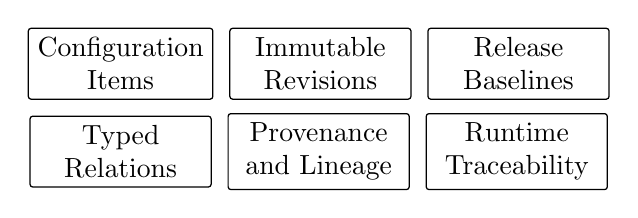
\begin{tikzpicture}[
            baseline,
            component/.style={
                draw,
                rounded corners=1pt,
                minimum width=23mm,
                minimum height=6mm,
                align=center,
                line width=0.45pt
            }
        ]
            \node[component] (aci) {Configuration\\Items};
            \node[component, right=2mm of aci] (revisions) {Immutable\\Revisions};
            \node[component, right=2mm of revisions] (baselines) {Release\\Baselines};

            \node[component, below=2mm of aci] (relations) {Typed\\Relations};
            \node[component, right=2mm of relations] (provenance) {Provenance\\and Lineage};
            \node[component, right=2mm of provenance] (runtime) {Runtime\\Traceability};
        \end{tikzpicture}
    };

    \draw[arrow] (projection) -- (acm);

    % ---------------------------------------------------------
    % Governance capabilities
    % ---------------------------------------------------------

    \node[layer, below=5mm of acm] (governance) {
        \textbf{Governance Capabilities}\\[4pt]
        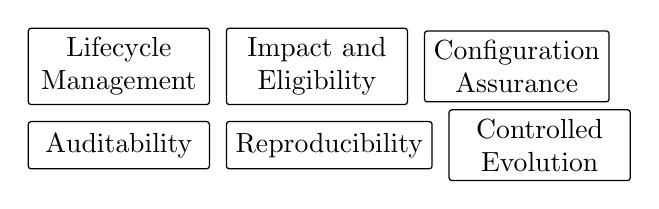
\begin{tikzpicture}[
            baseline,
            component/.style={
                draw,
                rounded corners=1pt,
                minimum width=23mm,
                minimum height=6mm,
                align=center,
                line width=0.45pt
            }
        ]
            \node[component] (lifecycle) {Lifecycle\\Management};
            \node[component, right=2mm of lifecycle] (impact) {Impact and\\Eligibility};
            \node[component, right=2mm of impact] (assurance) {Configuration\\Assurance};

            \node[component, below=2mm of lifecycle] (audit) {Auditability};
            \node[component, right=2mm of audit] (reproducibility) {Reproducibility};
            \node[component, right=2mm of reproducibility] (change) {Controlled\\Evolution};
        \end{tikzpicture}
    };

    \draw[arrow] (acm) -- (governance);

    \end{tikzpicture}

    \caption{Positioning of ACM with respect to heterogeneous agentic execution frameworks. Native configurations originating from explicit workflow graphs, metadata-driven orchestration, or delegation-based agent systems are semantically projected into a common framework-independent governance representation, allowing lifecycle management, assurance evaluation, provenance, traceability, and controlled evolution to operate independently of the originating execution framework.}
    \label{fig:acm_framework_positioning}
\end{figure}

\subsection{Contributions to Agentic Configuration Governance}
\label{sec:governance_contributions}

The contribution of ACM lies neither in introducing a new orchestration mechanism nor in extending the execution capabilities of existing agentic frameworks. Its primary contribution is to establish configuration governance as an explicit and framework-independent concern for agentic systems. From this perspective, ACM contributes at four complementary levels: representation, semantics, interoperability, and operational validation.

\subsubsection{A Framework-Independent Governance Representation}

The first contribution is a reference model that represents an agentic system as a governed configuration rather than as a collection of framework-specific runtime objects. The model introduces explicit configuration items, immutable revisions, typed relationships, provenance information, and release baselines. These abstractions provide a common vocabulary for describing the constituent elements of an agentic system and the dependencies that determine its effective configuration.

This representation extends established configuration-management principles to artifacts that are specific to agentic systems. In particular, it treats agents, prompts, tools, policies, models, workflows, and dynamically instantiated components as governable objects whose identity and evolution can be tracked independently. The resulting configuration is therefore not reduced to source code, deployment metadata, or execution traces. It is represented as an explicit and auditable object in its own right.

A central consequence of this model is the ability to distinguish logical identity from immutable revision identity. Successive revisions of the same configuration item preserve a stable conceptual identity while remaining individually addressable through exact revision identifiers and content digests. This distinction supports reproducibility, comparison, controlled replacement, and historical reconstruction without conflating an evolving artifact with one of its concrete states.

\subsubsection{Formal Governance Semantics}

The second contribution is the formalization of governance semantics over the reference model. ACM does not merely describe which artifacts exist; it defines how their governance states evolve and how local changes affect dependent configurations.

The lifecycle model specifies admissible transitions for configuration revisions, baselines, and runtime instances. Quality, assurance, impact, and eligibility are maintained as distinct dimensions rather than being collapsed into a single status. This separation prevents ambiguous interpretations such as treating a lack of evidence as proof of poor quality or propagating the lifecycle state of a dependency directly to its parent.

The propagation semantics further define how dependency changes, invalidated evidence, deprecated components, and runtime deviations influence the governance status of composite configurations. These effects are restrictive rather than destructive: a problematic dependency may block the promotion of a composite configuration without rewriting the intrinsic quality or lifecycle state of that composite. The model thereby preserves the provenance of governance decisions while supporting deterministic and explainable state computation.

The assurance model complements these semantics by linking governance conclusions to explicit evidence. Validation and approval are attached to exact revisions and scopes, allowing the system to distinguish directly assessed artifacts from conclusions inherited through assurance-relevant dependencies. Governance states can therefore be interpreted together with the evidence and rules from which they were derived.

\subsubsection{Framework-Independent Semantic Projection}

The third contribution is the separation between framework-specific extraction and framework-independent governance processing. Native configurations are translated into ACM through semantic projection, while the governance kernel operates exclusively on normalized ACM artifacts.

This architecture allows heterogeneous orchestration paradigms to be governed through a common representation. A graph-oriented framework may expose nodes and edges directly, whereas a role- and task-oriented framework may require part of its topology to be reconstructed from assignments and dependencies. ACM does not require these native representations to be structurally identical. It requires the projection to preserve the information needed for configuration governance and to make approximated or unavailable information explicit.

Framework independence should therefore be understood as independence of the governance model and processing semantics from a specific execution framework. The adapters remain framework-specific because they interpret native concepts. Once projection is complete, however, lifecycle validation, baseline construction, dependency analysis, assurance computation, runtime integration, and impact propagation no longer depend on the source framework.

This separation provides a basis for interoperability without imposing a common execution model. Frameworks retain their native orchestration semantics, while ACM supplies a shared governance representation above them.
The experimental evaluation further demonstrates that this interoperability extends beyond heterogeneous orchestration models to heterogeneous introspection regimes. The evaluated frameworks expose governance-relevant information through explicit execution graphs, metadata-assisted reconstruction, and delegation-oriented agent handoffs, respectively. By normalizing these complementary representations into a common ACM configuration graph, semantic projection isolates framework-specific extraction from governance processing, allowing identical governance semantics to be applied independently of the native introspection mechanism.

\subsubsection{Reference Operationalization and Evaluation}

The fourth contribution is the operationalization of the reference model through an executable implementation together with its experimental validation across three representative agentic frameworks. Beyond demonstrating implementability, the reference implementation provides a reproducible operational realization of the proposed governance semantics, including semantic projection, deterministic governance evaluation, runtime reconstruction, and quantitative impact analysis.

The LangGraph, CrewAI, and OpenAI Agents SDK adapters instantiate the semantic-projection boundary for three complementary execution and introspection paradigms. Their diversity does not establish universal applicability, but provides representative evidence that the ACM reference model accommodates heterogeneous configuration abstractions while preserving common governance semantics. 

The evaluation also contributes a structured validation methodology combining normative governance scenarios, automated tests, and semantic-preservation analysis. This methodology distinguishes successful representation from exact structural equivalence and records which governance-relevant properties are preserved, reconstructed, approximated, or unavailable. It therefore provides a more appropriate validation criterion for a reference model than conventional runtime-performance benchmarking. The experimental protocol further complements this qualitative validation with a dedicated quantitative assessment of deterministic impact propagation. Together, the two experimental campaigns demonstrate not only that heterogeneous configurations can be governed through a common reference model, but also that the resulting governance analyses remain reproducible and quantitatively consistent across complementary execution frameworks.

Taken together, these four contributions establish ACM as a configuration-governance abstraction positioned between agentic execution environments and higher-level operational or organizational governance processes. The reference model defines what is governed, the formal semantics define how governance states are computed, semantic projection connects heterogeneous frameworks to the model, and the reference implementation demonstrates that these mechanisms can be operationalized consistently.

\subsection{Practical Implications}
\label{sec:practical_implications}

Beyond its conceptual contribution, ACM has practical implications for the engineering and governance of agentic systems. By introducing an explicit and framework-independent configuration representation, the proposed model enables governance activities that are difficult to perform when configuration information remains fragmented across framework-specific abstractions.

The experimental evaluation indicates that these governance capabilities remain applicable across heterogeneous execution environments despite substantial differences in their native introspection mechanisms. Consequently, governance policies can be formulated over a stable configuration representation rather than being coupled to framework-specific execution abstractions. This separation is particularly important as agentic ecosystems continue to diversify and evolve.

A first implication concerns reproducibility. In current agentic ecosystems, reproducing a previous execution often requires reconstructing configurations from multiple heterogeneous artifacts, including prompts, workflow definitions, deployment parameters, runtime traces, and external resources. ACM addresses this fragmentation by associating executions with immutable configuration revisions and controlled release baselines. A governed execution can therefore be traced back to the exact configuration from which it originated, supporting reproducible experiments, regression analyses, and long-term maintenance. The experimental campaigns further indicate that reproducibility extends beyond immutable configuration snapshots. Equivalent governed representations, deterministic impact propagation, and identical governance outcomes were obtained across repeated executions and heterogeneous execution frameworks. These observations suggest that governance reproducibility depends primarily on the normalized ACM representation rather than on the native execution environment.

A second implication concerns auditability and traceability. Since governance decisions are explicitly linked to identified configuration revisions and supporting evidence, the provenance of a validation result or lifecycle transition becomes inspectable rather than implicit. This capability facilitates post-deployment analysis, compliance reporting, and forensic investigation by making configuration evolution transparent throughout the lifecycle of the system.

The explicit representation of dependencies also supports systematic change management. Instead of reasoning independently about prompts, agents, tools, or models, ACM represents these artifacts as interconnected configuration items whose relationships can be analyzed before modifications are promoted to a released baseline. Dependency-aware impact analysis provides early visibility into the potential consequences of configuration changes, reducing the likelihood of unintended regressions. The quantitative evaluation additionally suggests that governance-driven impact analysis may substantially reduce the configuration space requiring manual verification after a change. Rather than inspecting every potentially affected artifact, practitioners can focus their review on the governed impact set computed through deterministic propagation. Although the reported inspection reduction remains an experimental estimate rather than the outcome of a controlled user study, it illustrates the practical value of combining semantic dependency analysis with explicit governance relationships.


The proposed model also provides a common governance abstraction that may facilitate interoperability across heterogeneous execution environments. Organizations frequently combine multiple orchestration frameworks to address different operational requirements. By projecting these heterogeneous configurations into a shared governance representation, ACM enables governance policies to be expressed independently of the underlying execution technology while allowing each framework to preserve its native execution semantics. 
The evaluation also indicates that interoperability should not be interpreted solely as compatibility between orchestration frameworks. The successful projection of explicit workflow graphs, metadata-assisted orchestration, and delegation-based agent systems suggests that governance interoperability can also be achieved across heterogeneous introspection regimes, provided that governance-relevant semantics are preserved during semantic projection.

ACM may therefore contribute to the emerging AgentOps ecosystem by complementing existing observability and orchestration platforms with explicit configuration governance. Current operational platforms primarily focus on execution monitoring, tracing, evaluation, and operational metrics. ACM addresses a complementary concern by governing the configuration artifacts that determine how those executions are produced. Consequently, the model should be viewed as a governance layer that can coexist with, rather than replace, existing AgentOps and LLMOps infrastructures. 
From this perspective, ACM complements operational observability rather than competing with it. Execution-oriented platforms primarily describe what occurred during runtime, whereas ACM governs the configuration artifacts, dependencies, and assurance evidence that explain why a governed execution was possible. The combination of both perspectives provides a more complete governance foundation spanning configuration, execution, and evolution.

%%%%%%%%%%%%%%%%%%%%%%%%%%%%%%%%%%%%%%%%%%%%%%%%%%%%%%%%%%%%%%%%%%%%%%%%%%%%%%%%
\subsection{Limitations of the Current Reference Model}
\label{subsec:limitations}

The objective of ACM is to provide a framework-independent governance representation for the governance of agentic system configurations rather than an execution platform or an autonomous reasoning architecture. Accordingly, the current version focuses on representing governed configuration artifacts, their lifecycle, dependencies, provenance, assurance, and runtime conformance, while intentionally leaving the internal execution logic of agentic systems outside the scope of the reference model.

Table~\ref{tab:limitations_scope} summarizes the current coverage of ACM and the principal capabilities intentionally deferred to future work.

\begin{table}[t]
	\caption{Current scope of the ACM reference model.}
	\label{tab:limitations_scope}
	\centering
	\begin{tabular}{ll}
		
		\toprule
		
		Currently covered &
		Not yet covered \\
		
		\midrule
		
		Semantic projection &
		Distributed execution \\
		
		Configuration governance &
		Multi-agent planning strategies \\
		
		Immutable revision management &
		Learning and adaptation mechanisms \\
		
		Lifecycle semantics &
		Autonomous reasoning policies \\
		
		Dependency propagation &
		Self-modifying execution strategies \\
		
		Runtime provenance &
		Collective agent negotiation \\
		
		Assurance evaluation &
		Long-term memory management \\
		
		Deterministic replay &
		Continual learning \\
		
		Framework-independent governance &
		Native communication protocols (e.g., MCP, A2A) \\
		
		Cross-framework governance &
		Large-scale industrial validation \\
		
		\bottomrule
		
	\end{tabular}
	
	\end{table}

These limitations result from deliberate modeling decisions rather than technical constraints. ACM intentionally separates governance concerns from execution concerns in order to establish a stable and framework-independent governance layer. Integrating planning algorithms, reasoning strategies, learning mechanisms, or execution optimizations into the reference model would both increase its complexity and compromise the conceptual independence required for long-term interoperability.

Consequently, ACM treats reasoning engines, orchestration frameworks, planning modules, learning components, communication protocols, and other execution technologies as external systems whose observable configuration and runtime behavior can be represented and governed without prescribing their internal operation. ACM therefore specifies \emph{what} is governed---configuration revisions, baselines, dependencies, runtime observations, and assurance evidence---rather than \emph{how} autonomous agents reason, plan, negotiate, or learn.

This separation also preserves the stability of the governance model as agentic technologies evolve. New execution frameworks, orchestration paradigms, communication protocols, or reasoning techniques can be incorporated through semantic projection without modifying the governance semantics themselves. The evaluation presented in this paper should therefore be interpreted as validating the ability of ACM to represent and govern heterogeneous agentic configurations, not the correctness, efficiency, or intelligence of the underlying execution mechanisms.

Although the present evaluation demonstrates consistent governance semantics across three representative frameworks, these results should not be interpreted as establishing universal framework coverage. Additional validation across emerging execution environments, communication protocols, and industrial-scale deployments remains necessary to assess the broader applicability of the proposed governance model.

The experimental validation remains limited to the representative orchestration frameworks and configuration scales considered by the reference implementation. Although the reported results provide encouraging evidence regarding the generality of the proposed governance semantics across complementary introspection regimes, they remain confined to controlled experimental scenarios. Broader empirical validation involving additional execution frameworks, industrial-scale configurations, human-centered governance workflows, and emerging agent communication protocols will be required before stronger claims regarding general applicability can be made.

\subsection{Section Summary}

This discussion has positioned ACM as a framework-independent governance layer dedicated to the management of agentic system configurations throughout their lifecycle. Rather than introducing another orchestration framework or execution model, ACM separates governance from execution by providing a common semantic representation upon which lifecycle management, assurance evaluation, dependency analysis, provenance tracking, runtime traceability, and controlled evolution can be performed independently of the originating execution framework.

The experimental evaluation strengthens this positioning by demonstrating that the proposed governance semantics remain applicable across heterogeneous execution frameworks and complementary introspection regimes. Native configurations originating from explicit workflow graphs, metadata-assisted orchestration, and delegation-oriented agent systems are normalized through semantic projection into equivalent governed ACM representations. Together with the quantitative evaluation of deterministic impact propagation, these results indicate that governance can be expressed over a stable and framework-independent configuration model despite substantial differences in native execution abstractions.

The proposed reference model should therefore be viewed as a governance abstraction complementing existing AgentOps and agentic execution ecosystems rather than replacing them. By combining a unified configuration representation with formal governance semantics and reproducible operationalization, ACM establishes a common foundation for configuration governance while remaining intentionally independent of framework-specific orchestration mechanisms. The following section discusses the principal threats to the validity of the present study and the factors that should be considered when interpreting these results.

\section{Threats to Validity}
\label{sec:threats_validity}

The preceding sections presented the ACM reference model, its formal governance semantics, its operationalization through a reference implementation, and an experimental evaluation conducted across two heterogeneous agentic frameworks. Together, these elements provide evidence that the proposed model is internally consistent, operationally realizable, and capable of preserving governance semantics within the evaluated scope.

As with any reference model, however, these results must be interpreted within the boundaries of the assumptions, implementation choices, and experimental conditions that characterize the present study. The purpose of this section is therefore not to question the conceptual validity of ACM itself, but to identify the principal factors that may influence the interpretation, reproducibility, and generalization of the reported results.

Following established empirical research practice, we distinguish threats related to the scope of the reference model, the validation of its formal semantics, the internal validity of the experimental methodology, the external validity of the reported conclusions, and the reproducibility of the evaluation artifacts. These limitations define the current scope of evidence supporting ACM and naturally motivate the research directions discussed in the following section.

\subsection{Validity of the Reference Model}
\label{sec:validity_reference_model}

The primary objective of this study is to evaluate whether ACM provides a sufficiently expressive and framework-independent governance representation for representing and governing heterogeneous agentic system configurations. Consequently, the reported results should be interpreted as evidence supporting the proposed reference model within the scope of the evaluated frameworks rather than as a demonstration of universal applicability.

The evaluation intentionally considers two agentic frameworks exhibiting substantially different orchestration paradigms. LangGraph exposes an explicit graph-based execution model in which structural dependencies are directly represented, whereas CrewAI adopts a higher-level organization centered on agents, roles, tasks, and crews. Successfully projecting these heterogeneous representations into a common ACM configuration model provides initial evidence that the proposed abstractions are not tied to a single execution paradigm. Nevertheless, the evaluation remains limited to these two representative frameworks.

Other categories of agentic systems, including architectures relying on dynamic handoffs, highly decentralized coordination mechanisms, large-scale enterprise orchestration platforms, or future framework abstractions, have not yet been experimentally evaluated. Although the semantic projection architecture was explicitly designed to accommodate heterogeneous native representations, additional adapters and experimental studies are required before broader claims regarding framework independence can be established empirically.

Accordingly, the conclusions drawn from this study should be understood as demonstrating \emph{framework portability} across two structurally distinct orchestration paradigms rather than complete framework independence. The latter remains a design objective of the reference model whose broader empirical validation constitutes an important direction for future work.

\begin{table}[ht]
\centering
\caption{Scope of the Reference Model Validation}
\label{tab:validation_scope}
\begin{tabular}{p{5.1cm}cc}
\toprule
\textbf{Validation Aspect} & \textbf{Evaluated} & \textbf{Future Validation} \\
\midrule
Graph-based orchestration & \checkmark & \\
Role/task-based orchestration & \checkmark & \\
Framework-independent governance kernel & \checkmark & \\
Dynamic handoff architectures & & \checkmark \\
Enterprise-scale orchestration platforms & & \checkmark \\
Emerging agentic abstractions (e.g., skills) & & \checkmark \\
Additional execution frameworks & & \checkmark \\
\bottomrule
\end{tabular}
\end{table}

\subsection{Validity of the Formal Semantics}
\label{sec:validity_formal_semantics}

The governance semantics introduced in this work define the formal behavior of the ACM reference model through explicit lifecycle state machines, deterministic state propagation, assurance composition, and runtime governance rules. Unlike purely conceptual reference models, these semantics are operationalized by a reference implementation that executes the corresponding state computations, validation procedures, and propagation algorithms. Consequently, the reported experimental results validate not only the structural expressiveness of the reference model but also the practical executability of its governance semantics.

Nevertheless, the present study should not be interpreted as providing a formal proof of correctness of the proposed semantics. The mathematical definitions establish the intended behavior of the governance model, while the reference implementation demonstrates that these semantics can be operationalized consistently for the evaluated scenarios. This constitutes constructive evidence of correctness through implementation and experimentation rather than a formal verification of the underlying mathematical system.

Several theoretical properties therefore remain outside the scope of the current work. In particular, the study does not formally prove properties such as termination of the fixed-point propagation process, confluence under alternative evaluation orders, completeness of semantic reconstruction across arbitrary frameworks, or the minimality of the computed governance states. Although the deterministic implementation and the successful execution of the validation scenarios provide empirical confidence that these properties hold within the evaluated scope, they have not yet been established through formal verification techniques.

Accordingly, the formal semantics should be regarded as an executable semantic specification supported by experimental evidence rather than as a mathematically verified formal system. Extending ACM with machine-checked proofs or theorem-based verification constitutes an important direction for future research and would further strengthen the theoretical foundations of the proposed governance model.

\subsection{Generalizability}
\label{sec:generalizability}

The evaluation reported in this study provides initial evidence that the ACM reference model can represent and govern heterogeneous agentic systems originating from multiple orchestration paradigms. Nevertheless, the scope of the experimental validation remains intentionally limited and should not be interpreted as demonstrating universal applicability across the rapidly evolving ecosystem of agentic frameworks.

The experimental study covers two representative but structurally distinct orchestration paradigms. LangGraph represents explicit graph-based orchestration, where execution structure and dependencies are directly modeled, whereas CrewAI represents a higher-level role- and task-oriented orchestration model requiring semantic reconstruction during projection. The successful projection of both frameworks supports the claim that ACM can normalize heterogeneous configuration representations while preserving the governance information required by the reference model.

\begin{table}[t]
\caption{Scope of the Experimental Validation}
\label{tab:validation_scope}
\centering
\begin{tabular}{p{4.0cm}cc}
\toprule
\textbf{Agentic System Category} & \textbf{Evaluated} & \textbf{Future Work} \\
\midrule
Graph-based orchestration (LangGraph) & \checkmark & \\
Role/task-based orchestration (CrewAI) & \checkmark & \\
Dynamic handoff architectures & & \checkmark \\
Hierarchical multi-agent delegation & & \checkmark \\
Swarm-based coordination & & \checkmark \\
Pipeline-oriented orchestration & & \checkmark \\
Large-scale enterprise deployments & & \checkmark \\
Cross-organizational governance & & \checkmark \\
\bottomrule
\end{tabular}
\end{table}

However, the evaluation does not yet include several important categories of agentic systems. Frameworks relying on dynamic handoffs, hierarchical delegation, decentralized swarms, large-scale distributed execution, or pipeline-oriented component orchestration may expose governance abstractions that are not currently represented in the evaluation corpus. Although the ACM metamodel was intentionally designed to remain independent of framework-specific abstractions, additional projection rules or extensions may prove necessary when addressing such architectures.

Similarly, the current experiments were conducted on normative governance scenarios and a reference implementation intended to validate the expressiveness and operational feasibility of the proposed model. They do not constitute an evaluation of industrial deployments involving thousands of configuration items, heterogeneous execution infrastructures, long-running production systems, or continuously evolving organizational governance processes.

Consequently, the conclusions of this study should be interpreted as evidence that ACM provides a viable framework-independent governance model for the classes of agentic systems evaluated, rather than as proof of universal applicability to every existing or future orchestration framework. Extending the empirical validation to additional ecosystems and deployment contexts constitutes an important direction for future work.

%%%%%%%%%%%%%%%%%%%%%%%%%%%%%%%%%%%%%%%%%%%%%%%%%%%%%%%%%%%%%%%%%%%%%%%%%%%%%%%%
\subsection{Reproducibility and Replicability}
\label{subsec:reproducibility}

Reproducibility was a primary design objective throughout the development and
evaluation of ACM. To facilitate independent verification, the complete
experimental protocol is defined through declarative fixtures, normative
evaluation scenarios, deterministic governance rules, and an immutable event
model. These artifacts enable independent implementations to evaluate the same
governance properties under comparable experimental conditions.

An important characteristic of the evaluation methodology is that the
experimental scenarios are \emph{normative} rather than demonstrative. Each
scenario specifies a governance property that the reference implementation is
expected to verify, regardless of whether the evaluated execution represents a
valid or an invalid configuration. Consequently, successful evaluation does not
necessarily imply that the tested configuration is accepted by ACM; in many
cases, the expected outcome is precisely the detection of a governance
violation.

Several scenarios intentionally introduce invalid lifecycle transitions,
missing dependencies, unauthorized runtime behavior, or configuration drift.
The correct behavior of the governance kernel is therefore to detect, classify,
and report these inconsistencies according to the formal semantics defined by
the reference model. From this perspective, rejecting an invalid configuration
constitutes a successful execution of the corresponding normative scenario.

This distinction proved particularly valuable during the iterative development
of the reference implementation. Two scenarios (ACM-S02 and ACM-S20) initially
revealed inconsistencies between the normative specification and the prototype
implementation. Rather than invalidating the experimental methodology, these
results demonstrated its effectiveness as a validation mechanism: the observed
discrepancies led to refinements of the governance semantics before completion
of the evaluation campaign.

Replicability is further supported by the deterministic nature of the
governance kernel. Given identical configuration revisions, governance
policies, assurance evidence, and runtime events, repeated executions produce
equivalent governance states and identical compliance decisions. This property
holds independently of the probabilistic outputs generated by the underlying
LLMs because ACM governs configuration and execution semantics rather than
model inference itself.

The publication of the reference implementation, the declarative test
fixtures, the normative scenario suite, and the associated evaluation protocol
allows future implementations of ACM to reproduce the experimental campaign,
compare governance behaviors, and evaluate semantic equivalence independently
of the original prototype. The reproducibility objective of this work is
therefore not to reproduce a specific software implementation, but to enable
independent verification of the governance semantics defined by the ACM
reference model.

\begin{figure}[t]
    \centering
    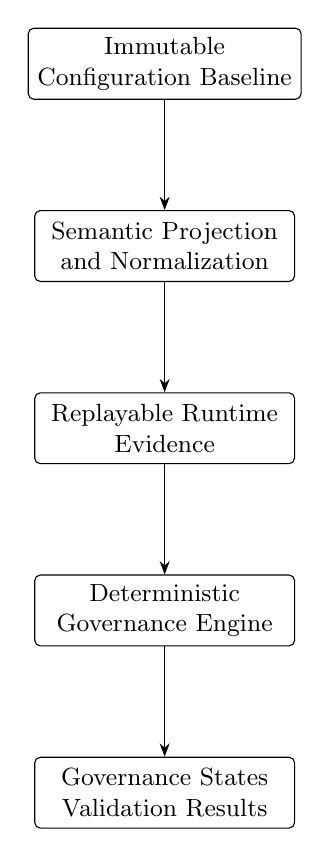
\begin{tikzpicture}[
    node distance=1.4cm,
    >=Stealth,
    box/.style={
        draw,
        rounded corners=2pt,
        align=center,
        minimum width=3.3cm,
        minimum height=0.9cm,
        font=\small
    }
]

\node[box] (baseline) {Immutable\\Configuration Baseline};

\node[box, below=of baseline] (projection) {Semantic Projection\\and Normalization};

\node[box, below=of projection] (runtime) {Replayable Runtime\\Evidence};

\node[box, below=of runtime] (engine) {Deterministic\\Governance Engine};

\node[box, below=of engine] (results) {Governance States\\Validation Results};

\draw[->] (baseline) -- (projection);
\draw[->] (projection) -- (runtime);
\draw[->] (runtime) -- (engine);
\draw[->] (engine) -- (results);

\end{tikzpicture}
    \caption{Deterministic governance pipeline supporting reproducibility and replicability. Immutable configuration baselines, semantic projection, replayable runtime evidence, and deterministic governance computation together enable independent reproduction of governance results without requiring deterministic LLM outputs.}
    \label{fig:reproducibility_pipeline}
\end{figure}

\subsection{Mitigation Strategies}
\label{sec:mitigation_strategies}

Although the preceding subsections identify several limitations affecting the present study, a number of methodological choices were deliberately adopted to reduce their impact on the reported results. Rather than attempting to maximize the breadth of the evaluation, the experimental methodology emphasizes internal consistency, deterministic governance semantics, and explicit separation between conceptual modeling, operationalization, and experimental validation.

First, the reference model was intentionally designed independently of any particular execution framework. The semantic projection architecture isolates framework-specific extraction mechanisms from the governance kernel, allowing the latter to remain unchanged across heterogeneous orchestration paradigms. This separation reduces implementation bias and facilitates the extension of the evaluation to additional frameworks without modifying the underlying governance semantics.

Second, the evaluation relies on normative governance scenarios rather than application-specific benchmarks. Each scenario targets a well-defined property of the reference model, such as lifecycle management, dependency propagation, assurance computation, baseline validation, or runtime governance. This scenario-driven methodology improves the traceability between the formal specification, the reference implementation, and the experimental evidence.

Third, reproducibility is reinforced through deterministic governance computation, immutable configuration revisions, canonical serialization, replayable runtime evidence, and automated validation procedures. These mechanisms ensure that governance outcomes depend exclusively on governed configurations and observed runtime events rather than on the stochastic behavior of the underlying language models.

In conclusion, this article deliberately distinguishes between the conceptual reference model, its formal governance semantics, the reference implementation, and the experimental evaluation. This separation avoids conflating theoretical contributions with implementation artifacts and allows future implementations to validate the same governance semantics independently of the current prototype.

Table~\ref{tab:mitigation_strategies} summarizes the principal threats identified in this section together with the corresponding mitigation strategies adopted throughout the study.

\begin{table}[t]
\caption{Summary of Threats and Mitigation Strategies}
\label{tab:mitigation_strategies}
\centering
\begin{tabular}{p{4.2cm}p{3.9cm}}
\toprule
\textbf{Threat} & \textbf{Mitigation Strategy} \\
\midrule
Limited framework coverage &
Evaluation across heterogeneous orchestration paradigms; framework-independent governance kernel. \\

Incomplete formal verification &
Executable formal semantics supported by deterministic implementation and normative validation scenarios. \\

Limited empirical generalization &
Conservative interpretation of results; explicit delimitation of the evaluation scope. \\

Implementation-dependent bias &
Separation between semantic projection, governance kernel, and framework adapters. \\

Experimental reproducibility &
Immutable revisions, replayable runtime events, canonical serialization, and automated validation suite. \\

Framework evolution &
Projection architecture designed to accommodate additional adapters without modifying the reference model. \\
\bottomrule
\end{tabular}
\end{table}

\subsection{Section Summary}
\label{sec:threats_summary}

The objective of this section has been to delimit the scope within which the conclusions of the present study should be interpreted. The identified threats do not challenge the internal consistency of the ACM reference model nor the coherence of its governance semantics. Instead, they primarily concern the breadth of the experimental validation, the current level of formal verification, and the extent to which the reported results can be generalized across the rapidly evolving landscape of agentic systems.

The experimental methodology intentionally favors methodological rigor over exhaustive coverage by combining a framework-independent governance representation, executable governance semantics, deterministic validation procedures, and reproducible experimental artifacts. Within this scope, the reported results provide credible evidence supporting the feasibility and expressiveness of the proposed governance model while avoiding claims that extend beyond the evaluated configurations.

These limitations naturally define the next stage of the research agenda. In particular, extending the empirical validation to additional orchestration paradigms, strengthening the formal verification of the governance semantics, and broadening the ecosystem supported by semantic projection represent logical continuations of the present work. These directions are discussed in the following section.

\section{Future Work}
\label{sec:future_work}

The ACM reference model introduced in this paper constitutes an initial step toward a framework-independent approach to the governance of agentic systems. The proposed metamodel, governance semantics, reference implementation, and experimental evaluation collectively demonstrate the feasibility of this approach within the scope considered in the present study. At the same time, the limitations identified in the previous section highlight several opportunities for extending both the theoretical foundations and the practical applicability of ACM.

Future research therefore naturally follows three complementary directions. The first concerns the evolution of the reference model itself to accommodate emerging abstractions while preserving its governance principles. The second focuses on strengthening the empirical and theoretical validation of the proposed semantics through broader experimental studies and formal verification. The long-term perspective is to position ACM as a common governance layer capable of interoperating with the rapidly expanding ecosystem of agentic development, deployment, and observability platforms.

\subsection{Extension of the Reference Model}
\label{sec:future_reference_model}

The reference model presented in this paper intentionally focuses on the minimal set of governance concepts required to represent heterogeneous agentic systems independently of their execution framework. This design choice favors conceptual stability and limits the number of core abstractions to those introducing distinct governance semantics. Nevertheless, the rapid evolution of agentic ecosystems will inevitably lead to the emergence of new configuration artifacts, interaction patterns, and execution abstractions that may require additional modeling capabilities.

A primary direction for future research is therefore the controlled evolution of the ACM metamodel while preserving its foundational design principles. Rather than continuously introducing framework-specific concepts into the core model, future extensions should remain guided by semantic necessity: a new abstraction should only become part of the reference model if it introduces governance properties that cannot be represented through the existing concepts and relationships. This principle preserves the framework independence of ACM while avoiding unnecessary growth of the metamodel.

An important example concerns reusable composite capabilities that are increasingly appearing under different names across modern agentic platforms, such as skills, reusable workflows, capability modules, or packaged execution components. Although these constructs differ in their implementation details, they frequently encapsulate existing governed artifacts—including prompts, tools, models, policies, workflows, and external resources—rather than introducing fundamentally new governance semantics. Consequently, many of these emerging abstractions can already be represented through semantic projection as governed composite configuration items without requiring modifications to the ACM core.

An additional extension concerns Retrieval-Augmented Generation (RAG) systems, which are becoming a fundamental building block of modern agentic applications. Rather than introducing a dedicated governance abstraction, ACM can represent RAG pipelines through the composition of existing configuration items, including embedding models, retrieval policies, vector indexes, knowledge repositories, prompt definitions, and retrieval components. This representation enables immutable versioning of the complete retrieval configuration, explicit provenance of derived vector indexes, and governance of retrieval policies independently of the underlying storage technology. Consequently, ACM can govern the evolution of retrieval-augmented systems without embedding retrieval-specific concepts into its core metamodel.

Another important direction concerns self-learning or continuously adaptive agents. Such systems challenge traditional configuration management because parts of their operational behavior may evolve autonomously through accumulated experience, parameter adaptation, or long-term memory updates. Extending ACM to distinguish immutable governed configurations from controlled runtime knowledge evolution would enable adaptive systems to remain auditable while preserving reproducibility of approved configurations. Future work should therefore investigate governance semantics capable of representing learning artifacts, adaptation boundaries, and evidence associated with autonomous configuration evolution.

Finally, the increasing adoption of interoperability protocols and workflow orchestration platforms, including Model Context Protocol (MCP), Agent-to-Agent (A2A) communication, and low-code orchestration environments such as n8n, provides another opportunity for extending the reference model. Rather than incorporating protocol-specific abstractions, ACM can represent these ecosystems through semantic projection of communication endpoints, external services, orchestration workflows, and interaction contracts into governed configuration items. This approach preserves the framework-independent nature of the reference model while enabling configuration governance across heterogeneous execution environments and emerging interoperability standards.

Future extensions may also address governance capabilities that extend beyond the scope of the current reference model. Examples include distributed governance across multiple organizations, federated configuration repositories, cross-system dependency management, richer policy composition mechanisms, and governance of long-lived autonomous ecosystems whose configuration evolves continuously over time. These extensions would broaden the applicability of ACM while preserving the separation between configuration governance and execution that constitutes one of its central architectural principles.

Ultimately, the long-term evolution of ACM should prioritize conceptual stability over feature accumulation. As with mature reference models in software engineering, the objective is not to mirror every innovation introduced by individual frameworks, but rather to identify the stable governance abstractions that remain applicable despite the continuous evolution of execution technologies. This philosophy enables the reference model to evolve incrementally while maintaining interoperability, explainability, and long-term sustainability.

\subsection{Broader Framework Validation}
\label{sec:future_framework_validation}

The empirical evaluation presented in this paper intentionally focuses on two representative orchestration paradigms in order to demonstrate the feasibility of framework-independent configuration governance. Although the successful semantic projection of LangGraph and CrewAI provides encouraging evidence supporting the proposed reference model, broader validation across the rapidly evolving landscape of agentic systems remains an essential research direction.

Future work should therefore extend the experimental corpus to additional execution frameworks exhibiting different orchestration principles and configuration abstractions. In particular, frameworks supporting dynamic handoffs, hierarchical delegation, event-driven coordination, decentralized multi-agent collaboration, or long-running autonomous workflows would provide valuable opportunities to evaluate the expressiveness of the ACM metamodel under substantially different execution models.

Beyond execution frameworks themselves, validation could also incorporate complementary components of the emerging AgentOps and LLMOps ecosystem. Provenance platforms, observability infrastructures, evaluation frameworks, and deployment management systems increasingly expose governance-relevant metadata that could naturally participate in semantic projection. Studying the integration of ACM with such platforms would provide additional evidence regarding the ability of the reference model to serve as a common governance layer across heterogeneous operational environments.

Another important direction concerns empirical validation at industrial scale. The current experiments intentionally emphasize semantic correctness rather than operational scalability. Future studies should therefore evaluate ACM on large agentic systems involving hundreds or thousands of governed configuration items, long-lived execution histories, continuously evolving baselines, and collaborative governance processes distributed across multiple development teams. Such evaluations would provide quantitative evidence regarding scalability, governance overhead, and operational usability in realistic production environments.

Ultimately, extending the experimental validation is not intended merely to increase the number of supported frameworks. Rather, it aims to progressively strengthen the empirical evidence supporting the central hypothesis of this work: that governance semantics can remain stable despite the continuous evolution of agentic execution technologies.

\subsection{Formal Verification of Governance Semantics}
\label{sec:future_formal_verification}

The governance semantics introduced in this paper are defined through a formal operational specification and validated through deterministic execution of the reference implementation. While this approach demonstrates the practical executability of the proposed semantics, it does not constitute a formal mathematical proof of their correctness. Establishing such guarantees represents an important direction for future research.

One immediate objective concerns the verification of the fixed-point propagation algorithm underlying governance state computation. Formal proofs could establish properties such as termination, determinism, convergence toward a unique governance state, and independence from evaluation order. Demonstrating these properties would strengthen confidence that governance decisions remain stable regardless of implementation details or execution strategies.

A second research direction involves the formal analysis of the lifecycle semantics themselves. The lifecycle state machines, dependency propagation rules, assurance composition mechanisms, and runtime governance semantics could be expressed within a formal verification framework in order to prove invariants such as transition consistency, absence of contradictory governance states, preservation of dependency constraints, and correctness of state propagation under arbitrary configuration topologies.

Beyond individual algorithms, future work may investigate the formal specification of the ACM reference model as a complete governance system. Model-checking techniques, temporal logic, theorem proving, or specification languages dedicated to distributed systems could be employed to verify global properties of the governance semantics and to detect inconsistencies automatically during the evolution of the reference model. Such approaches would complement the current implementation-based validation with machine-verifiable correctness guarantees.

Formal verification would facilitate the development of independent ACM implementations. By providing mathematically specified governance semantics rather than relying solely on behavioral equivalence with the reference implementation, future implementations could demonstrate conformance through proof of semantic equivalence instead of implementation similarity. This evolution would represent an important step toward establishing ACM as a stable and implementation-independent governance specification.

\subsection{Toward an Agentic Configuration Ecosystem}
\label{sec:future_ecosystem}

The rapid maturation of agentic software engineering has led to the emergence of a rich ecosystem of complementary technologies dedicated to development, deployment, observability, evaluation, provenance, and operational governance. Rather than replacing these existing tools, ACM is intended to provide a framework-independent governance layer capable of connecting heterogeneous components through a common semantic representation of governed configuration artifacts.

A promising direction for future research therefore consists in studying the integration of ACM with broader AgentOps and LLMOps ecosystems. Modern observability platforms increasingly collect execution traces, evaluation results, model usage metrics, cost information, and provenance metadata that constitute valuable inputs for governance processes. Conversely, governance decisions produced by ACM could enrich these platforms with lifecycle status, assurance levels, configuration lineage, dependency analysis, and compliance information, providing a higher semantic level for operational monitoring.

Another important perspective concerns the integration of ACM with software engineering infrastructures. Continuous integration and deployment pipelines, software configuration management systems, artifact repositories, and supply-chain security mechanisms already manage the lifecycle of conventional software assets. Extending these infrastructures to incorporate governed agentic configuration items would enable unified governance across both traditional software components and AI-native artifacts while preserving traceability throughout the complete development lifecycle.

Beyond tooling integration, future work may explore the definition of interoperable governance services exposing standardized interfaces for semantic projection, configuration validation, governance state computation, and provenance exchange. Such services would facilitate the development of heterogeneous toolchains in which execution frameworks, observability platforms, deployment systems, and governance engines cooperate while remaining independently evolvable.

Ultimately, the long-term objective is to establish ACM not as another execution platform, but as a common semantic governance layer capable of interconnecting the diverse technologies that increasingly compose modern agentic software ecosystems.

\subsection{Standardization Perspectives}
\label{sec:future_standardization}

The absence of a common vocabulary and shared governance abstractions currently represents one of the principal obstacles to interoperability across agentic systems. While execution frameworks continue to evolve rapidly, equivalent concepts are frequently described using framework-specific terminology, making configuration exchange, governance portability, and comparative evaluation unnecessarily difficult.

The ACM reference model represents an initial step toward addressing this fragmentation by proposing a framework-independent conceptual vocabulary together with formally defined governance semantics. Although the present work does not aim to establish a standard, it provides a structured foundation upon which future community discussions regarding interoperable governance models may build.

Future research may therefore investigate the definition of standardized exchange formats for governed configuration items, semantic projection interfaces, governance evidence, provenance information, and lifecycle metadata. Such specifications would facilitate interoperability between heterogeneous execution frameworks while allowing governance information to remain portable independently of implementation technologies. Likewise, standardized conformance criteria could enable independent implementations to demonstrate semantic compatibility with the ACM reference model while preserving implementation freedom.

The maturation of ACM may also benefit from collaboration with broader software engineering and artificial intelligence communities working on software configuration management, software supply-chain security, provenance, and AI governance. Aligning ACM with existing standards whenever appropriate would facilitate its integration into established engineering practices while reducing duplication of concepts that are already well understood in adjacent disciplines.

Ultimately, the long-term ambition is not to standardize a particular implementation, but to encourage convergence toward a shared governance language for agentic systems towards an agentic configuration ecosystem. By separating governance semantics from execution technologies, ACM provides a stable conceptual foundation that could evolve collaboratively as the agentic landscape continues to mature. Such convergence would improve interoperability, reproducibility, auditability, and long-term sustainability across heterogeneous agentic platforms. Such anglobal agentic ecosystem, including ACM, could progressively evolve toward interoperable configuration exchange and, ultimately, contribute to future standardization efforts for governed agentic systems.

\section{Conclusion}
\label{sec:conclusion}

The rapid evolution of agentic software engineering has fundamentally transformed the role of configuration artifacts. Prompts, tools, execution graphs, policies, models, runtime state, and provenance have become first-class engineering assets whose governance can no longer rely solely on traditional software configuration management practices. At the same time, the increasing diversity of orchestration frameworks has introduced heterogeneous configuration abstractions, making governance difficult to reproduce, audit, and compare across platforms.

This paper introduced Agentic Configuration Management (ACM), a framework-independent governance representation for the governance of agentic systems. Rather than proposing another execution framework, ACM separates governance semantics from execution technologies through a unified representation of governed configuration items, immutable revisions, semantic relationships, deterministic lifecycle management, assurance semantics, and runtime governance. This separation enables heterogeneous agentic systems to be represented within a common governance model while preserving the flexibility of existing orchestration frameworks.

Beyond the conceptual contribution, the paper demonstrated that the proposed semantics can be operationalized through a reference implementation and evaluated using representative orchestration paradigms. The experimental results show that heterogeneous agentic configurations can be semantically projected into a common governance representation while preserving the information required for deterministic governance decisions. Although the current evaluation remains intentionally limited in scope, it provides initial empirical evidence supporting the feasibility of framework-independent configuration governance for agentic systems.

More broadly, this work argues that governance should become an explicit architectural layer of agentic software engineering rather than an implementation-specific concern embedded within individual execution frameworks. By introducing a common vocabulary, formally defined governance semantics, and a framework-independent governance representation, ACM establishes a foundation upon which future research can investigate interoperability, formal verification, scalable governance, and standardized configuration management practices for increasingly autonomous AI systems.

Ultimately, the contribution of ACM is not to prescribe how agentic systems should execute, but to provide a stable semantic foundation for governing how they are specified, versioned, validated, traced, and evolved. As agentic ecosystems continue to diversify, such a separation between execution and governance may become an essential prerequisite for building reproducible, auditable, interoperable, and trustworthy AI systems.


\bibliographystyle{IEEEtran}
\bibliography{references}
\end{document}

